\chapter{时间-空间网络的构建与拓展表示}\label{ch:时间-空间网络的构建与拓展表示}

在传统的网络问题上,路段上的路段阻抗常被视作是一个常数,也称为静态路网。而对于现实情况的交通路网,路段阻抗函数通常受到多重影响因素的共同作用,需要考虑随机性和时变性等问题,因此路段阻抗函数应该为时间的函数,即d=f(t)。并且在动态网络中,各路段和相关节点之间是相互作用的,在网络中某个节点或路段发生故障,其造成的影响不仅仅是该条路段或该节点,而是一个区域的路段和节点。

为了刻画交通网络的动态性和网络中路段和节点之间的相关作用关系,本章节将主要对比地介绍一般的物理交通网络表示和离散的动态交通网络的时间-空间表示以及对网络拓扑结构中节点和路段关系约束的拓展表示。


\section{物理交通网络表示}\label{sec:物理交通网络表示}

在交通运输规划和管理领域中,物理交通网络一般表示为有向图G=(V, E, W) 。其中$V=\{1, 2, \dots,n\}$表示网络中节点的集合,
而$E=\{(i,j) \in V \times V\}$表示边的集合,其中(i,j)表示从节点i到节点j的有向路段。路段的数量用m表示,使用$W=\{w_{ij} (t)|(i,j)\in E\}$表示随时间变化的路段行程时间集合。
在如图\ref{fig:fig2}所示的交通网络中,有6个节点和13条路段,每条路段都有相对应的权重,即表示路段行程时间。
\begin{figure}[H] %H为当前位置,!htb为忽略美学标准,htbp为浮动图形
    \centering %图片居中
    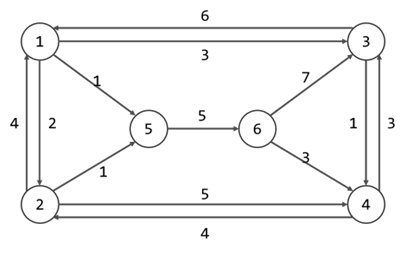
\includegraphics[width=0.7\textwidth]{png/图片2 简单静态交通网络示例} %插入图片,[]中设置图片大小,{}中是图片文件名
    \caption{简单静态交通网络示例} %最终文档中希望显示的图片标题
    \label{fig:fig2} %用于文内引用的标签
\end{figure}

对于静态网络,经典的最短路算法可以很高效的计算出网络中的最优路径。
然而对于动态网络,例如动态随机网络则不能很好的求解,
如图\ref{fig:fig3}所示。驾驶者从节点1处出发,可以经过路径A:$1 \to 3 \to 6$或路径B:$1\to 2\to 3\to 6$这两条路径到达节点6。
由于两条路径中到达节点3的到达时间不相同,即两条路径中$3\to 6$的出发时间不相同,因此对于同一路段产生了不同的路段行程时间。
\begin{figure}[H] %H为当前位置,!htb为忽略美学标准,htbp为浮动图形
    \centering %图片居中
    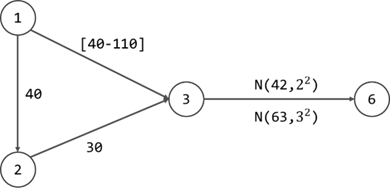
\includegraphics[width=0.7\textwidth]{png/图片3 动态随机网络} %插入图片,[]中设置图片大小,{}中是图片文件名
    \caption{动态随机交通网络示例} %最终文档中希望显示的图片标题
    \label{fig:fig3} %用于文内引用的标签
\end{figure}

假设一个具体的场景:驾驶者在7:00从节点1出发,路段$1 \to 3$的行程时间服从U(40,110)的均匀分布,
而路段$1\to 2\to 3$的总行程时间为固定的40+30=70,假设在节点内部同样存在时间的消耗,例如8:00---8:30节点3处的行程时间消耗为7,
而在其他时间行程时间消耗为1,在8:15之前出发的情况下,路段(3,6)的路段形成时间服从正态分布$N(63,3^2)$,
而8:15之后出发的话路段服从正态分布$N(42,2^2)$。对于路径13的期望最短行程时间为75,
而路径$1\to 2\to 3$的最短行程时间为70,但是$1\to 3\to 6$的期望最短行程时间为124,而$1\to 2\to 3\to 6$的期望最短行程时间为140。
可以看出,动态最短路问题已经不满足Bellman条件:每条最短路径的子路径也是最短路径,即若节点i到节点j的最短路径中经过节点k,
则节点i到节点k的最短路径是节点i到节点j的最短路径的前缀。同样,Bellman条件也不适用于时间-空间网络中最短路的求解。


\section{时间-空间交通网络表示}\label{sec:时间-空间交通网络表示}
与上面介绍的静态交通网络相比,时间-空间网络能够更好地描述出现实世界中交通网络的动态变化性质,
例如在一天早晚高峰时段路段的阻抗会呈现出双峰分布,而在相邻的时间段内路段阻抗值差异较小,
如图\ref{fig:fig4}所示。由于交通流具有明显的周期性,通常来说可以以一天或一周为一个周期进行分析,
对于路段的阻抗信息,可以根据该区域内路段的历史阻抗信息,
采用时间序列分析的方法来预测将来相应时间段内的路段阻抗。

\begin{figure}[H] %H为当前位置,!htb为忽略美学标准,htbp为浮动图形
    \centering %图片居中
    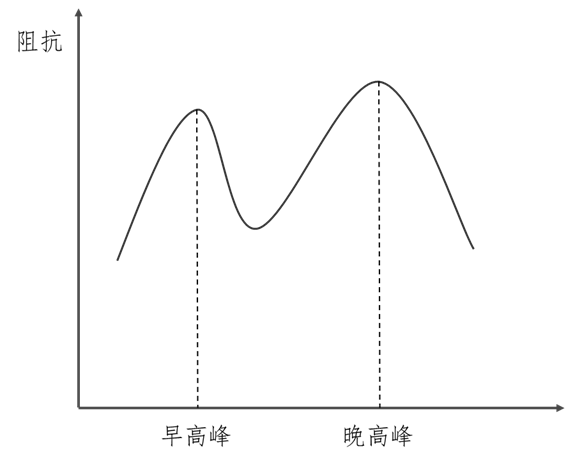
\includegraphics[width=0.7\textwidth]{png/图片4 路段阻抗分布} %插入图片,[]中设置图片大小,{}中是图片文件名
    \caption{路段阻抗分布} %最终文档中希望显示的图片标题
    \label{fig:fig4} %用于文内引用的标签
\end{figure}

时间-空间网络表示可以根据阻抗函数和时间的函数关系分为连续网络和离散网络,
根据前面对交通流的分析,交通网络中在一定时间内的路段阻抗值相差不大,
因此接下来将使用离散时间-空间网络建模,同时离散网络也对问题作出一定程度的简化且方便计算机求解,
可以使得动态网络转变为相对应的静态网络进行求解,对路段阻抗离散化处理之后的结果如图\ref{fig:fig5}所示。

\begin{figure}[H] %H为当前位置,!htb为忽略美学标准,htbp为浮动图形
    \centering %图片居中
    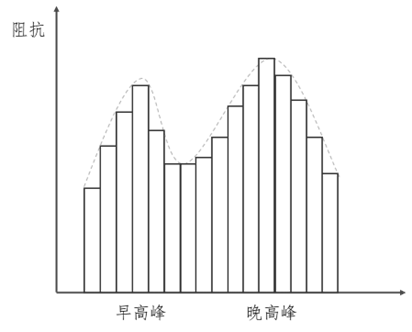
\includegraphics[width=0.7\textwidth]{png/图片5 路段阻抗离散化处理结果} %插入图片,[]中设置图片大小,{}中是图片文件名
    \caption{路段阻抗离散化处理结果} %最终文档中希望显示的图片标题
    \label{fig:fig5} %用于文内引用的标签
\end{figure}

上面已经对单条路段的阻抗函数进行了离散化处理,
而对于时间-空间路网则需要对路网中所有的路段进行离散化处理,
常用形式有时间拓展图和时间集聚图。时间聚集图通过一个序列来表示路段上的阻抗,
占用的内存相比于时间拓展图而言更少,因此对于规模相对较大的网络而言处理速度更快,效率更高。

\begin{figure}[H] %H为当前位置,!htb为忽略美学标准,htbp为浮动图形
    \centering %图片居中
    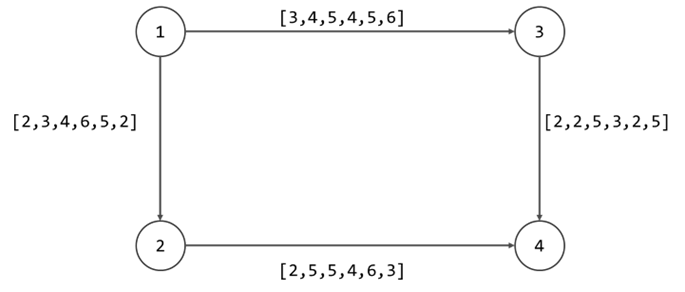
\includegraphics[width=0.7\textwidth]{png/图片6 时间聚集图} %插入图片,[]中设置图片大小,{}中是图片文件名
    \caption{时间聚集图} %最终文档中希望显示的图片标题
    \label{fig:fig6} %用于文内引用的标签
\end{figure}
在如图\ref{fig:fig6}所示的时间聚集图中,将每条路段的阻抗划分为6个切片,
分别代表6个不同时段的路段阻抗值。时间聚集图虽然可以相对高效的求解网络最短路,
但是不如时间拓展图直观,网络实际拓扑结构也不清晰。
若将图\ref{fig:fig6}所示的时间聚集图展开为时间拓展图, 则如图\ref{fig:fig7}所示。
时间拓展图会使得原本简单的网络拓扑变得异常复杂,网络中节点的数目根据切片数量成倍数增长,
即$N=kN_0$,其中$N_0$是时间拓展图中节点的数量,k为切片数量,N为时间拓展图中节点的数量。

\begin{figure}[H] %H为当前位置,!htb为忽略美学标准,htbp为浮动图形
    \centering %图片居中
    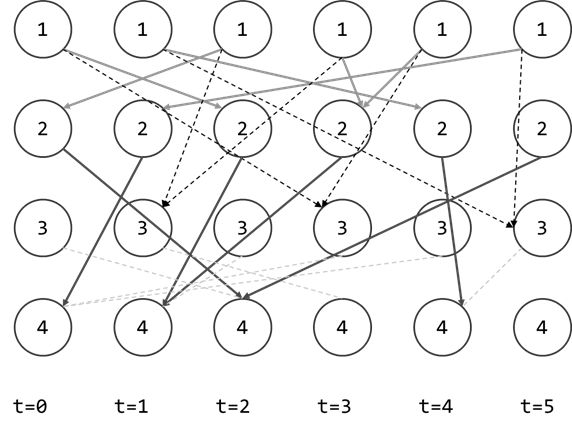
\includegraphics[width=0.7\textwidth]{png/图片7 时间拓展图} %插入图片,[]中设置图片大小,{}中是图片文件名
    \caption{时间拓展图} %最终文档中希望显示的图片标题
    \label{fig:fig7} %用于文内引用的标签
\end{figure}

对于考虑从任意时间,任意节点出发的一个网络,将出发时刻视作t=0,出发节点视作节点1,
此时可以将时间拓展图简化为时间-空间交通网络状态图,如图\ref{fig:fig8}所示。
时间-空间状态相比于时间拓展图的存储效率更高,适用于路段交通流量差异较大的实时计算中使用。

\begin{figure}[H] %H为当前位置,!htb为忽略美学标准,htbp为浮动图形
    \centering %图片居中
    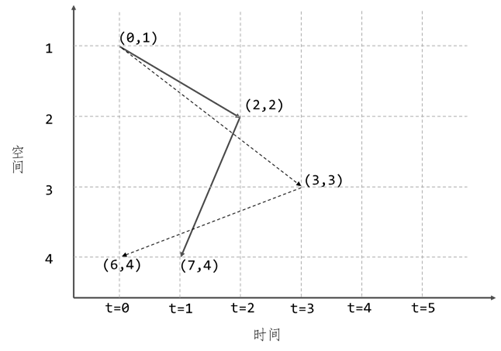
\includegraphics[width=0.7\textwidth]{png/图片8 时间-空间状态图} %插入图片,[]中设置图片大小,{}中是图片文件名
    \caption{时间-空间状态图} %最终文档中希望显示的图片标题
    \label{fig:fig8} %用于文内引用的标签
\end{figure}
同时,一条实际的物理路径可能对应时间-空间交通网络中的多条不同时刻出发和不同时刻到达的路径。
如图\ref{fig:fig8}所示,从节点1到节点4仅在t=0时刻便分别对应$1\to 2\to 4$和$1\to 3\to 4$两条路径。
因此对所研究的问题,我们可以在传统的静态最短路网的基础上,
针对驾驶者的出发时刻和出行决策建立动态的最短路模型,具体建模过程将于第四章进行具体介绍。


\section{交通网络节点拓扑结构的拓展表示}\label{sec:交通网络节点拓扑结构的拓展表示}
在上面的时间-空间网络中,我们已经可以在构建的模型中很好地体现出交通网络的动态性和周期性,
但是却没有考虑到节点阻抗造成的影响。在很多场景下,节点阻抗对网络路径造成的影响是不可忽略的,
例如在交叉口左转、右转、直行,又或者在不同的地铁线路之间换乘,
因此我们需要通过一定的方法将节点阻抗转变为路段阻抗,从而完成对问题形式上的统一,
方便对问题进行求解。下面以图\ref{fig:fig9}所示南京地铁线路图为例,介绍如何在交通网络的拓扑结构中对节点阻抗进行描述。

\begin{figure}[H] %H为当前位置,!htb为忽略美学标准,htbp为浮动图形
    \centering %图片居中
    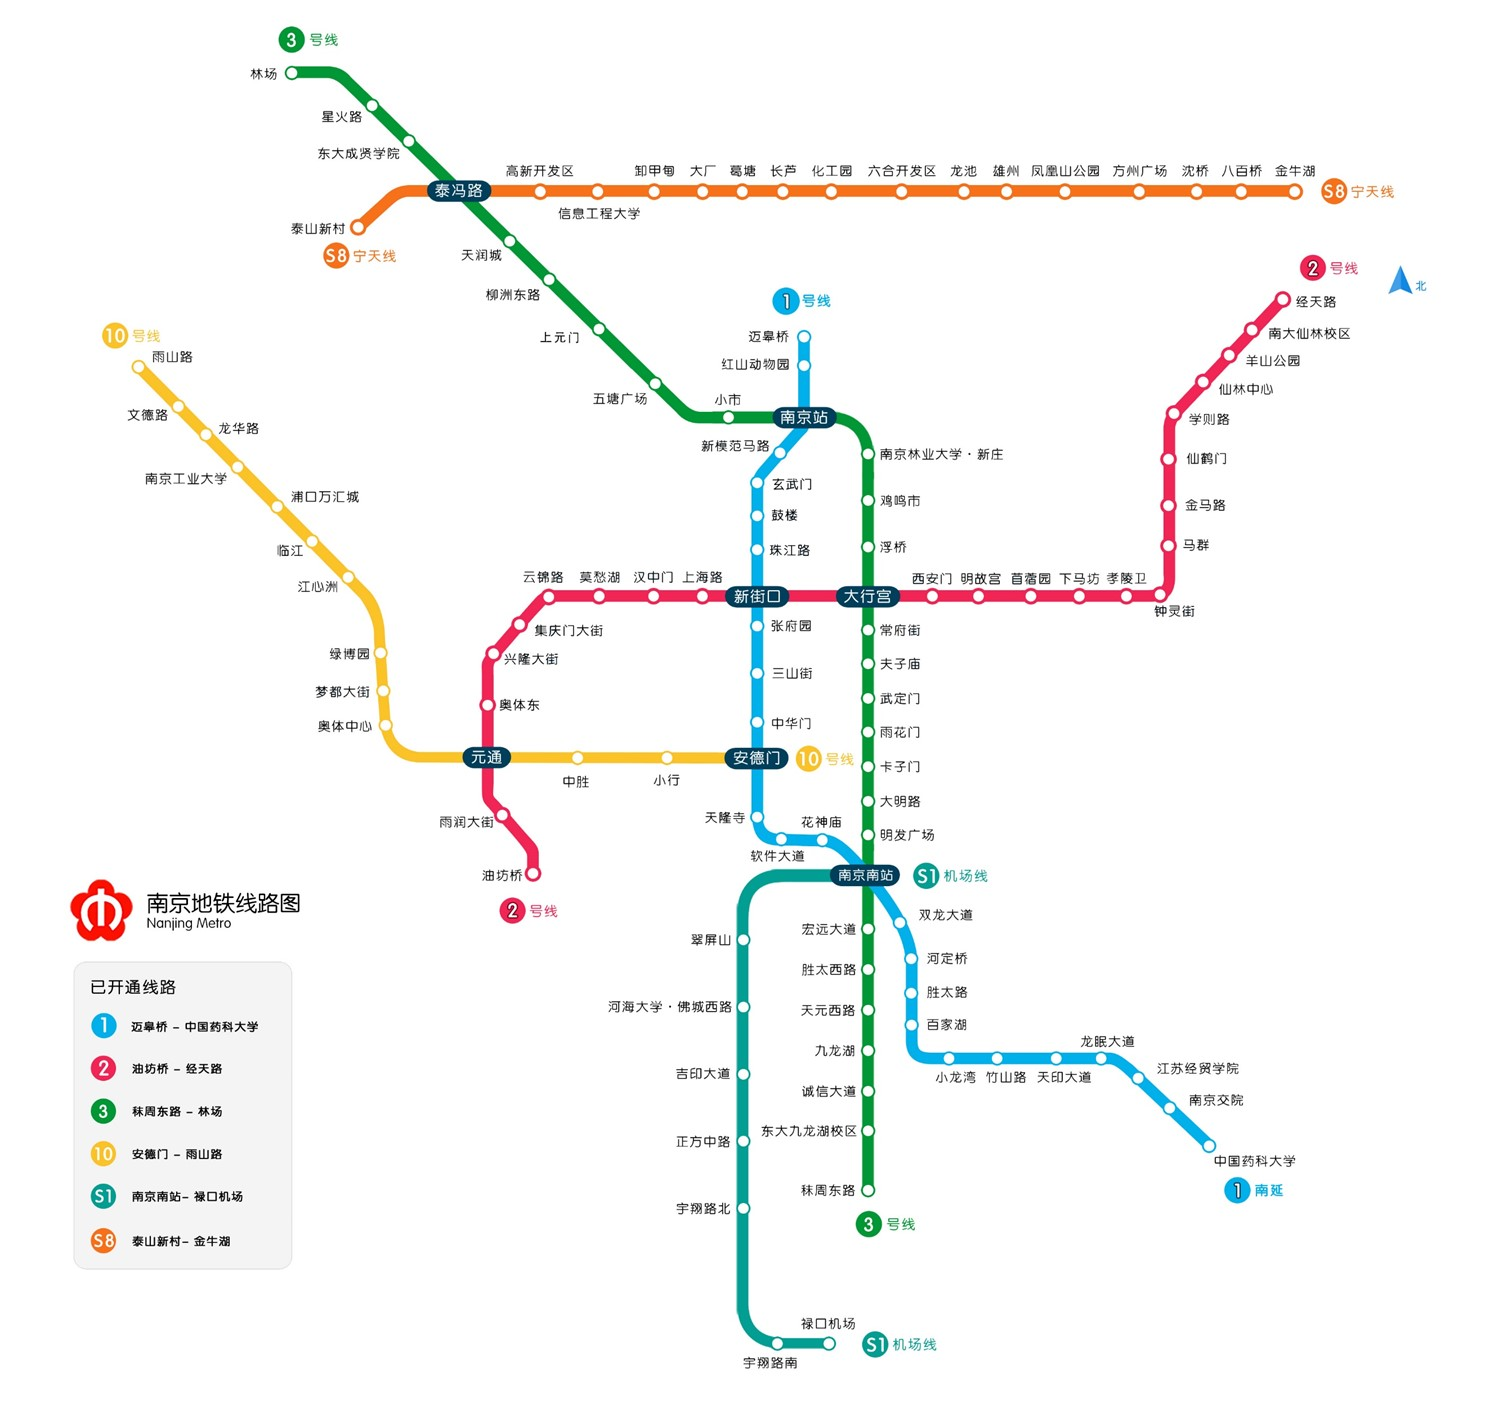
\includegraphics[width=0.7\textwidth]{png/图片9 南京地铁线路图} %插入图片,[]中设置图片大小,{}中是图片文件名
    \caption{南京地铁线路图} %最终文档中希望显示的图片标题
    \label{fig:fig9} %用于文内引用的标签
\end{figure}

以地铁1号线和地铁3号线的换乘站(南京南站)为例,
上面所述的时间-空间网络状态图中在南京南站乘客换乘的时间没有考虑,
因此需要对节点进行拓展,采用拆点法的思想,将节点拆分为多对出发节点和到达节点,
在换乘线路之间添加惩罚项,而没有换乘行为的路段则认为对应一条阻抗值为0的路段,如图\ref{fig:fig10}所示。

\begin{figure}[H] %H为当前位置,!htb为忽略美学标准,htbp为浮动图形
    \centering %图片居中
    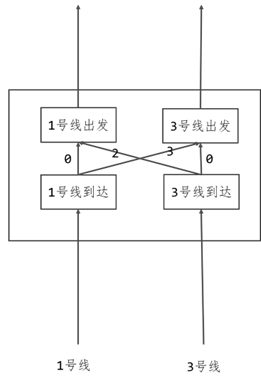
\includegraphics[width=0.5\textwidth]{png/图片10 换乘站结点的拓展表示} %插入图片,[]中设置图片大小,{}中是图片文件名
    \caption{换乘站结点的拓展表示} %最终文档中希望显示的图片标题
    \label{fig:fig10} %用于文内引用的标签
\end{figure}

综上所述,在时间-空间网络结合交通网络有着自己独特的流量特点,时间-空间交通网络呈现周期性的变化特点,且在微观上交通流的变化是连续的,而在宏观上交通流的变化是离散的,呈现出双峰分布的特点。
因此时间空间网络中的多条最短路问题可以通过时间拓展图的处理方法转化为静态网络中多个源点序列到多个汇点序列的多条最短路问题。
时间-空间拓展网络如图\ref{fig:fig11}所示。

\begin{figure}[H] %H为当前位置,!htb为忽略美学标准,htbp为浮动图形
    \centering %图片居中
    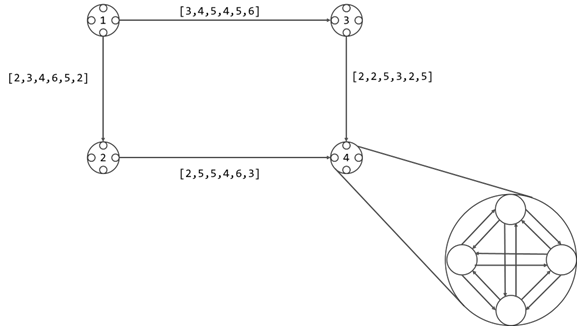
\includegraphics[width=0.7\textwidth]{png/图片11 节点拓展的时间-空间网络状态图} %插入图片,[]中设置图片大小,{}中是图片文件名
    \caption{节点拓展的时间-空间网络状态图} %最终文档中希望显示的图片标题
    \label{fig:fig11} %用于文内引用的标签
\end{figure}